% Zadnja posodobitev: 14. 1. 2022
\documentclass[twoside,11pt]{article}
\usepackage[slovene]{babel}
\usepackage[utf8]{inputenc}
\usepackage{graphicx}
\usepackage[frame]{matrika}
\usepackage{mathtools}
\usepackage{epstopdf}
\usepackage{units}
% Po potrebi se lahk dodajo drugi standardni paketi, ki ne spreminjajo izgleda dokumenta


\usepackage{tikz}
\usetikzlibrary{positioning, 
                arrows.meta,                % arrow tips
                intersections,              % find intersection between paths
                spath3} % split and transform paths



\begin{document}

\MAT{1}{11}{2024}
\naslov{Brownovo gibanje}

\avtor{Anej Rozman}

\institucija{Fakulteta za matematiko in fiziko \\ Univerza v Ljubljani}

\klasifikacija{~} 
\izvlecek{V članku motiviramo idejo Brownovega gibanja in podamo njegovo matematično definicijo. 
    Predstavimo nekaj osnovnih lastnosti in rezultatov, kot simetričnost Brownovega gibanja,  }
\title{Brownian motion}
\abstract{}

\glava\baselineskip=14.5pt

\smallskip

\section{Uvod}

Določeni posebni primeri slučajnih procesov so skozi zgodovino doživeli obsežen
matematični razvoj. Brownovo gibanje je najbolj znano in zgodovinsko prvo, ki je bilo 
temeljito raziskano. Kot fizičen pojav je
bilo Brownovo gibanje odkrito s strani angleškega botanika Roberta Browna leta 1827.
Matematični opis tega pojava je bil prvič izpeljan iz fizikalnih zakonov s strani 
Einsteina leta 1905. Od takrat je področje doseglo znaten napredek. Fizikalno teorijo 
so nadalje izpopolnili Fokker, Planck, Ornstein in drugi. Matematična 
teorija je počasneje napredovala, ker je natančen matematični opis modela postavljal 
težave, medtem ko so bila nekatera vprašanja, na katera so fiziki iskali odgovore na
podlagi tega modela, precej preprosta in intuitivna. Veliko odgovorov je bilo
pridobljenih heuristično s strani Bachelierja v njegovi disertaciji leta 1900.
Prvo jasno matematično formulacijo teorije pa je Wiener podal v svoji
disertaciji leta 1918 in kasnejših člankih, zato je alternativno ime za 
Brownovo gibanje Wienerjev proces. Brownovo gibanje je primer kontinuiranega 
časa, kontinuiranega prostora stanj Markovskega procesa, ki se danes skupaj z 
njegovimi posplošitvami pojavlja na številnih področjih kot so biologija, finance in kot
že omenjena, fizika. V članku se bomo
osredotočili na matematično izpeljavo osnovnega Brownovega gibanja na $\mathbb{R}$ 
ter njegove lastnosti in ne na uporabo v zgoraj omenjenih področjih.




\pagebreak
\section{Motivacija in definicija Brownovega gibanja}

Kot Robert Brown si za motivacijo oglejmo naključno gibanje delca v $\mathbb{R}^2$.
Smiselno bi bilo, da zahtevamo, da se gibanje začne v koordinatnem izhodišču. Želeli bi tudi, da so 
poti oziroma trajektorije delca zvezne, saj nam nenadni skoki nebi pomagali pri opisovanju 
pojava.  

\begin{figure}[h]
    \centering
    \begin{tikzpicture}
      \draw[->] (-1,0) -- (6,0) node[right] {$x$};
      \draw[->] (0,-1) -- (0,4) node[above] {$y$};
  
      \draw[thick,blue] plot[smooth,tension=0.8] coordinates {(0,0) (1,2) (2,1) (3.3, 2.6) (3,3) (2.5,2) (5,2) (6,3.2)};

      \filldraw[black] (6,3.2) circle (1pt);

      \node[above ,black] at (6,3.2) {$\left(B^x_{t}, B^y_{t}\right)$};
    \end{tikzpicture}

    \caption{Primer trajektorije Brownovega gibanja v xy-ravnini.}
    \label{fig:slika1}
\end{figure}

\noindent
Označimo z $\left(B^x_{t}, B^y_{t}\right)$ položaj delca v času $t \geq 0$. Ker se delec v vse 
smeri giblje z enako verjetnostjo, bo pričakovana vrednost pozicije enaka $\mathbb{E}\left[(B_t^x, B_t^y)\right] = (0, 0).$
Smiselno bi bilo privzeti, da so premiki delca med časi $0 < t_1 < t_2 < \dots < t_n < \infty$ med seboj neodvisni, torej, 
da gibanje med časom $0$ in $t_1$ (razen tega kje gibanje začnemo) ne vpliva na gibanje med časom $t_1$ in $t_2$ in tako naprej.
Matematično to zapišemo, da so vektorji $(B^x_{t_2}, B^y_{t_2}) - (B^x_{t_1}, B^y_{t_1}), \ \dots, (B^x_{t_n}, B^y_{t_n}) - (B^x_{t_{n-1}}, B^y_{t_{n-1}})$
med seboj neodvisni. Če to velja vidimo, da je $\left(B^x_{t}, B^y_{t}\right)$ vsota neodvisnih prirastkov. Po centralnem 
limitnem izreku bi torej pričakovali, da je vektor $\left(B^x_{t}, B^y_{t}\right)$ normalno porazdeljen.
Spomnimo se, da je slučajna spremenljivka $X$ normalno porazdeljena s pričakovano vrednostjo $\mu$ in varianco $\sigma^2$, če
je njena gostota porazdelitve enaka
$$
    f_X(x) = \frac{1}{\sqrt{2\pi\sigma^2}}\exp\left(-\frac{(x-\mu)^2}{2\sigma^2}\right).
$$
Zaradi neodvisnosti prirastkov bo tudi $\text{Var}(B_t^x) = \text{Var}(B_t^y) = t$, torej odvisna le od tega koliko 
časa opazujemo delec.
Te opazke nas privedejo do definicije Brownovega gibanja na $\mathbb{R}$, kjer bi jih radi matematično karakterizirali.

\begin{definicija}
    Slučajnemu procesu $(B_t)_{t\geq 0}$ definiranem na verjetnostnem prostoru $(\Omega, \mathcal{F}, \mathbb{P})$
    z vrednostmi v $\mathbb{R}$ pravimo \textit{Brownovo gibanje}, če 
    zadošča naslednjim pogojem:
    \begin{enumerate}
        \item $\mathbb{P}(B_0 = 0) = 1$,
        \item trajektorije $(B_t)_{t\geq0}$ so $\mathbb{P}$-skoraj gotovo zvezne,
        \item proces $\left(B_t\right)_{t \geq 0}$ ima neodvisne prirastke t.j. za $0 \leq t_1 < t_2 < \dots < t_n < \infty$ so slučajne spremenljivke
            $B_{t_2} - B_{t_1}, \ B_{t_3} - B_{t_2}, \ \dots, \ B_{t_n} - B_{t_{n-1}}$ med seboj neodvisne. 
        \item Za $ 0 \leq s < t < \infty$ je $B_t - B_s \sim N(0, t-s)$.
    \end{enumerate}
\end{definicija}
        
Prvo vprašanje, ki se nam porodi, je, ali sploj obstajta verjetnostni prostor 
in slučajni proces, ki zadoščata zgornjim zahtevam. Odgovor je pritrdilen in ga 
podamo v obliki izreka.

\begin{izrek}
    Obstaja verjetnostni prostor $(\Omega, \mathcal{F}, \mathbb{P})$ in
    izbira slučajnih spremenljivk $B_t : \Omega \to \mathbb{R}$ za $t \geq 0$,
    ki ustrezajo definiciji Brownovega gibanja.
\end{izrek}

\begin{dokaz}
    Dokaz izreka je precej tehničen in nezanimiv za namen članka, zato ga bomo izpustili.
     Lahko ga najdemo v \cite{1}. $\hfill \square$
\end{dokaz}


Od sedaj naprej bomo privzeli, da je $(B_t)_{t\geq 0}$ Brownovo gibanje vedno definirano na 
verjetnostnem prostoru $(\Omega, \mathcal{F}, \mathbb{P})$ in se nanj (razen po potrebi) ne 
bomo sklicevali. Priročno bo v mislih držati sliko \ref{fig:slika2}.

\begin{figure}[h]
    \centering
    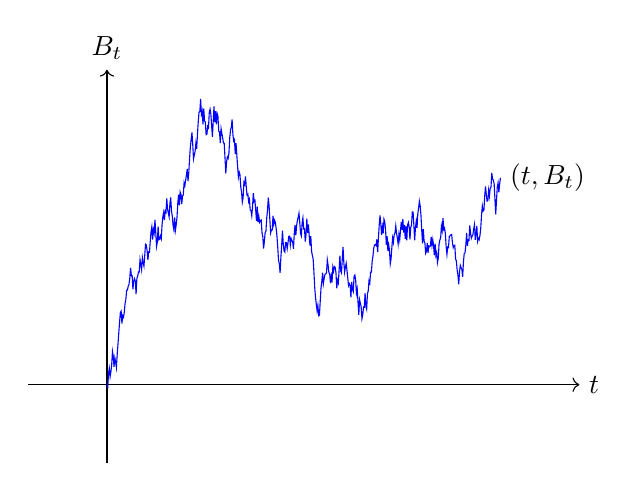
\begin{tikzpicture}
        \pgfmathsetseed{941}
      \draw[->] (-1,0) -- (6,0) node[right] {$t$};
      \draw[->] (0,-1) -- (0,4) node[above] {$B_t$};

      \draw[blue] (0,0)
      \foreach \x in {1,...,500}
      { -- ++(0.01,rand*-0.2)
      }
      node[right, black] {$(t,B_t)$};

    \end{tikzpicture}
    \caption{Primer trajektorije eno-dimenzionalnega Brownovega gibanja.}
    \label{fig:slika2}
\end{figure}

\section{Lastnosti}

\subsection{Osnovne lastnosti}

Poglejmo si nekaj osnovnih lastnosti Brownovega gibanja, ki nam bodo prišle prav v nadaljevanju 
članka.

\begin{trditev}
    Naj bo $(B_t)_{t\geq 0}$ Brownovo gibanje in $0 \leq s < t < \infty$. Potem velja
    $$
        Cov(B_t, B_s) = s
    $$
\end{trditev}

\begin{dokaz}
    Ker je $B_t - B_s \sim N(0, t-s)$, sledi
    $$
        Cov(B_t, B_s) = Cov(B_s + B_t - B_s, B_s) = Cov(B_s, B_s) + Cov(B_t - B_s, B_s) = s + 0 = s.
    $$
    $\hfill \square$
\end{dokaz}

Za nadaljevanje bomo potrebovali naslednjo trditev iz teorije mere.

\begin{trditev}
     Če velja $\mathbb{E}\left[f(X)g(X)\right] = \mathbb{E}\left[f(X)\right]\mathbb{E}\left[g(X)\right]$. za vsak par 
     omejenih zveznih funkcij $f, g$, potem sta $X$ in $Y$ neodvisni.
\end{trditev}

\begin{definicija}
    Naj bo $X$ slučajna spremenljivka na verjetnostnem prostoru $(\Omega, \mathcal{F}, \mathbb{P})$
    in $\mathcal{G} \subseteq \mathcal{F}$ pod-$\sigma$-algebra. $X$ je \textit{neodvisna}
    od $\mathcal{G}$, če za vsako omejeno zvezno funkcijo $f$ velja
    $$
        \mathbb{E}\left[f(X)1_G\right] = \mathbb{E}\left[f(X)\right]\mathbb{P}(G)
    $$
    za vsak $G \in \mathcal{G}$.
\end{definicija}

\begin{definicija}
    Naj bo $(B_t)_{t\geq 0}$ Brownovo gibanje. S $\mathcal{F}_t$ 
    označimo $\sigma$-algebro generirano z$ \sigma(B_s \mid 0\leq s \leq t)$. 
    Družini $(\mathcal{F}_t)_{t\geq 0}$ pravimo \textit{Brownova filtracija}.
\end{definicija}

\begin{izrek}
    Za vsak fiksen $t \geq 0$ je proces $\{B_{t+s}-B_t\mid s\geq 0\}$ Brownovo gibanje neodvisno 
    od $\mathcal{F}_t$.
\end{izrek}

\begin{dokaz}
    Naj bo $0 \leq t < \infty$ in $0 \leq s_1 < s_2 < \dots < s_n < \infty$. 
    Potem je $B_{t+s_1} - B_t, \ B_{t+s_2} - B_{t+s_1}, \ \dots, \ B_{t+s_n} - B_{t+s_{n-1}}$ 
    neodvisen od $\mathcal{F}_t$, saj je neodvisen od $B_t$ in je $\mathcal{F}_t$ generiran z 
    $B_t$. Torej je $\{B_{t+s}-B_t\mid s\geq 0\}$ neodvisen od $\mathcal{F}_t$.
    $\hfill \square$
\end{dokaz}

\begin{definicija}
    Naj bo $(\mathcal{F}_t)_{t\geq0}$ filtracija. Slučajna spremenljivka $T: \Omega \rightarrow [0, \infty)\cup \{\infty\}$ 
    je \textit{čas ustavljanja} glede na filtracijo $(\mathcal{F}_t)_{t\geq0}$, če je za vsak $t \in \mathbb{R}$ dogodek $\{T \leq t\} \in \mathcal{F}_t$.
\end{definicija}

\begin{primer}
    Naj bo $(B_t)_{t\geq0}$ Brownovo gibanje in $a \in \mathbb{R}$. Potem je
    $$
        T_a = \inf\{t \geq 0 \mid B_t = a\}
    $$
    čas ustavljanja glede na filtracijo $(\mathcal{F}_t)_{t\geq0}$.
\end{primer}

\begin{figure}[h]
    \centering
    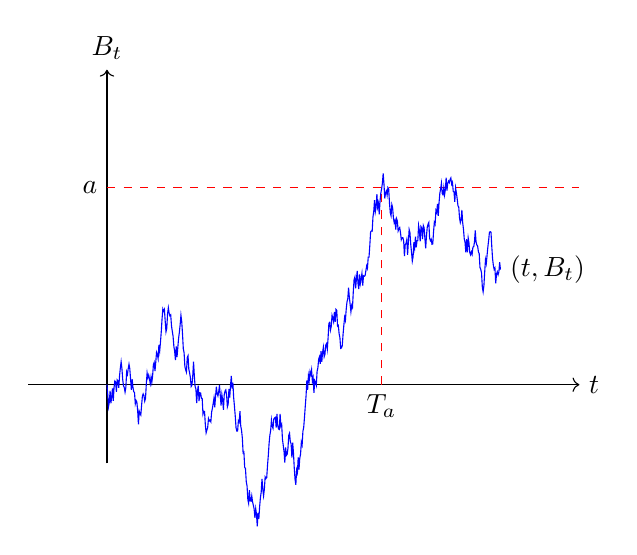
\begin{tikzpicture}
        \pgfmathsetseed{8}
        \draw[->] (-1,0) -- (6,0) node[right] {$t$};
        \draw[->] (0,-1) -- (0,4) node[above] {$B_t$};
        \draw[red, dashed] (0,2.5) -- (6,2.5);
        \draw[black] (0, 2.5) node[left] {$a$};
        \draw[red, dashed] (3.485,0) -- (3.485,2.5);
        \draw[black] (3.485, 0) node[below] {$T_a$};
  
        \draw[blue] (0,0)
        \foreach \x in {1,...,500}
        { -- ++(0.01,rand*-0.2)
        }
        node[right, black] {$(t,B_t)$};

    \end{tikzpicture}
    \caption{Primer realizacije $T_a$.}
    \label{fig:slika3}
\end{figure}



\begin{trditev}
    Naj bo $(B_t)_{t\geq 0}$ Brownovo gibanje. Potem velja, da je simetrično,
    torej $-(B_{t})_{t\geq0}$ je tudi Brownovo gibanje.
\end{trditev}

\subsection{Krepka lastnost Markova}
Pokažimo, da je za Brownovo gibanje velja krepka lastnost Markova. Torej, če 
v nekem trenutku ustavimo proces in ga gledamo od te točke dalje, bo neodvisen od
dotedanjega gibanja ter bo ponovno Brownovo gibanje.

\begin{izrek}
    Naj bo $(B_t)_{t\geq 0}$ Brownovo gibanje in $T$ čas ustavljanja, da velja $\mathbb{P}(T<\infty )=1$.
    Definiramo proces $B^*_s = B_{T + s} - B_T$ za $s\geq0$. Potem je $(B^*_s)_{s\geq0}$ Brownovo
    gibanje, neodvisno od $\mathcal{F}_T$.
\end{izrek}

\begin{dokaz}
    trivial duh $\hfill \square$
\end{dokaz}

Če izrek ponazorimo s sliko.

\begin{figure}[h]
    \centering
    \begin{tikzpicture}
        \pgfmathsetseed{10}
        \draw[->] (-1,0) -- (6,0) node[right] {$t$};
        \draw[->] (0,-1) -- (0,4) node[above] {$B_t$};
        \draw[->, green] (2.3, 1.5) -- (6, 0);
        \draw[->, green] (2.3, 1.5) -- (2.3, 4);
        \draw[red, dashed] (3.485,0) -- (3.485,2.5);
        \draw[black] (3.485, 0) node[below] {$T$};
  
        \draw[blue] (0,0)
        \foreach \x in {1,...,230}
        { -- ++(0.01,rand*-0.2)
        }

        \draw[red] (2.3, 1.5)
        \foreach \x in {1,...,270}
        { -- ++(0.01,rand*-0.2)
        }
        node[right, black] {$(t,B_t)$};
    \end{tikzpicture}
    \caption{Krepka lastnost Markova.}
    \label{fig:slika4}
\end{figure}



\subsection{Princip zrcaljenja}


\begin{figure}[h]
    \centering
    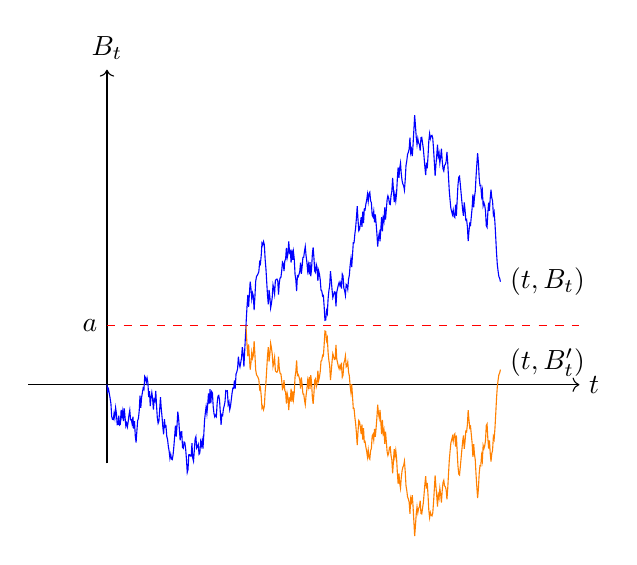
\begin{tikzpicture}
    \pgfmathsetseed{952}
    \draw[->] (-1,0) -- (6,0) node[right] {$t$};
    \draw[->] (0,-1) -- (0,4) node[above] {$B_t$};
    \draw[black] (0, 0.75) node[left] {$a$};

    \draw[spath/save=horiz, red, dashed] (0,0.75) -- (6,0.75);

    \draw[blue, spath/save=squiggly] (0,0)
      foreach \x in {1,...,500}{
         -- ++(0.01,rand*-0.2) 
         }
      node[right, black] {$(t,B_t)$};

        \draw[
            draw=orange,
            spath/.cd,
            split at intersections with={squiggly}{horiz},
            remove components={squiggly}{1},
            use={squiggly, transform={yshift=1.5cm,yscale=-1}},
            ] node[anchor=base west] {$(t,B'_t)$};

    \end{tikzpicture}
    \caption{Primer zrcaljenja Brownovega gibanja.}
    \label{fig:slika5}
\end{figure}



\begin{thebibliography}{99}

\bibitem{1} S. Roman, \emph{Introduction to mathematics of finance : from risk management to options pricing}, Science \textbf{269} (2004), 238--275. 
\bibitem{2} W. Ketterle, D.M. Kurn, D.S. Durfee, N.J. van Druten, M.R. Andrews, M.-O. Mewes in K.B. Davis, \emph{Bose-Einstein Condensation in a Gas of Sodium Atoms}, Physics Review Letters \textbf{75} (1995), 3969--3973. 


\end{thebibliography}

\end{document}
